\title{Getting Started}

% Begin the content of the page
\subsection{Getting Started}
Getting started with Edward is easy.

\subsubsection{Quick Installation}
To install the latest stable version, run

\begin{lstlisting}[language=Java]
pip install edward
\end{lstlisting}

To install the latest development version, run

\begin{lstlisting}[language=Java]
pip install -e "git+https://github.com/blei-lab/edward.git#egg=edward"
\end{lstlisting}

See the \href{troubleshooting.html}{troubleshooting page} for detailed
installation instructions.


\subsubsection{Your first Edward program}

Probabilistic modeling in Edward uses a simple language of
random variables. Here we will show a Bayesian neural network: a neural
network with a prior distribution on its weights.
(This example is abridged; full source
\href{https://github.com/blei-lab/edward/blob/master/examples/getting_started_example.py}
{here}.)

First, simulate a toy dataset of 50 observations with a cosine relationship.
\begin{lstlisting}[language=Python]
import numpy as np

x_train = np.linspace(-3, 3, num=50)
y_train = np.cos(x_train) + norm.rvs(0, 0.1, size=50)
\end{lstlisting}
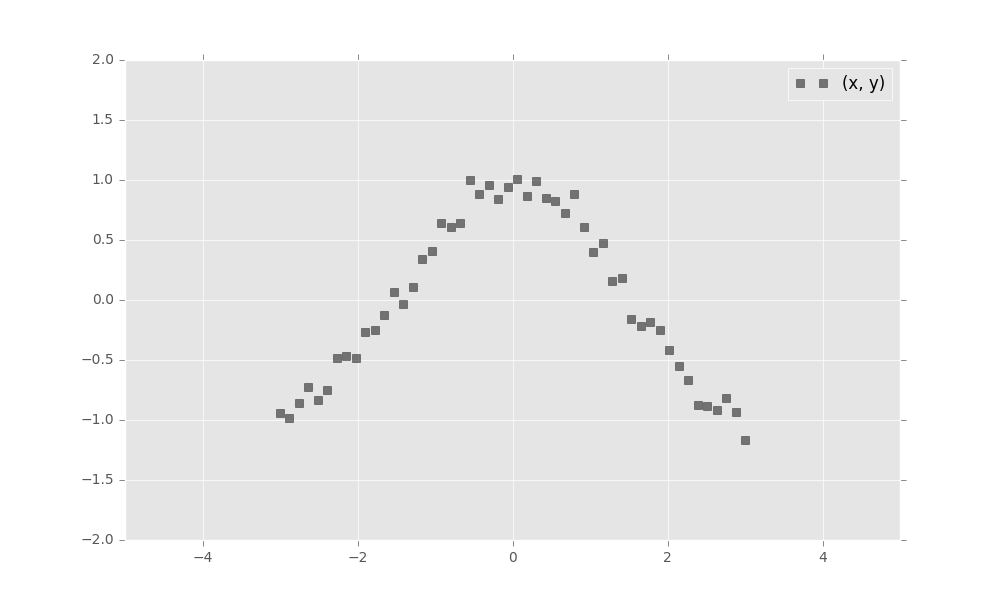
\includegraphics[width=700px]{images/getting-started-fig0.png}
Next, define a Bayesian neural network with one hidden layer.
\begin{lstlisting}[language=Python]
import tensorflow as tf
from edward.models import Normal

W_0 = Normal(mu=tf.zeros([1, 2]), sigma=tf.ones([1, 2]))
W_1 = Normal(mu=tf.zeros([2, 2]), sigma=tf.ones([2, 2]))
W_2 = Normal(mu=tf.zeros([2, 1]), sigma=tf.ones([2, 1]))
b_0 = Normal(mu=tf.zeros(2), sigma=tf.ones(2))
b_1 = Normal(mu=tf.zeros(2), sigma=tf.ones(2))
b_2 = Normal(mu=tf.zeros(1), sigma=tf.ones(1))

x = tf.convert_to_tensor(x_train, dtype=tf.float32)
y = Normal(mu=neural_network(x, W_0, W_1, W_2, b_0, b_1, b_2),
           sigma=0.1)
\end{lstlisting}

Next, make inferences about the model from data.
Edward focuses on variational inference. Specify a normal
approximation over the weights and biases.
\begin{lstlisting}[language=Python]
from edward.models import Normal

qW_0 = Normal(mu=tf.Variable(tf.random_normal([1, 2])),
              sigma=tf.nn.softplus(tf.Variable(tf.random_normal([1, 2]))))
qW_1 = Normal(mu=tf.Variable(tf.random_normal([2, 2])),
              sigma=tf.nn.softplus(tf.Variable(tf.random_normal([2, 2]))))
qW_2 = Normal(mu=tf.Variable(tf.random_normal([2, 1])),
              sigma=tf.nn.softplus(tf.Variable(tf.random_normal([2, 1]))))
qb_0 = Normal(mu=tf.Variable(tf.random_normal([2])),
              sigma=tf.nn.softplus(tf.Variable(tf.random_normal([2]))))
qb_1 = Normal(mu=tf.Variable(tf.random_normal([2])),
              sigma=tf.nn.softplus(tf.Variable(tf.random_normal([2]))))
qb_2 = Normal(mu=tf.Variable(tf.random_normal([1])),
              sigma=tf.nn.softplus(tf.Variable(tf.random_normal([1]))))
\end{lstlisting}
Defining \texttt{tf.Variable} allows the variational factors'
parameters to vary. They are initialized randomly.  The standard
deviation parameters are constrained to be greater than zero according
to a
\href{https://en.wikipedia.org/wiki/Rectifier_(neural_networks)}{softplus}
transformation.

Now, run mean-field variational inference. Infer the model's latent variables
conditional on data using the variational distribution.
We specify \texttt{1000} iterations.
\begin{lstlisting}[language=Python]
import edward as ed

data = {y: y_train}
inference = ed.MFVI({W_0: qW_0, b_0: qb_0,
                     W_1: qW_1, b_1: qb_1,
                     W_2: qW_2, b_2: qb_2}, data)
inference.run(n_iter=1000)
\end{lstlisting}

Finally, criticize the model fit. Bayesian neural networks define a
distribution over neural networks, so let's do a graphical check. Draw
neural networks from the inferred model and visualize how well it
fits the data.

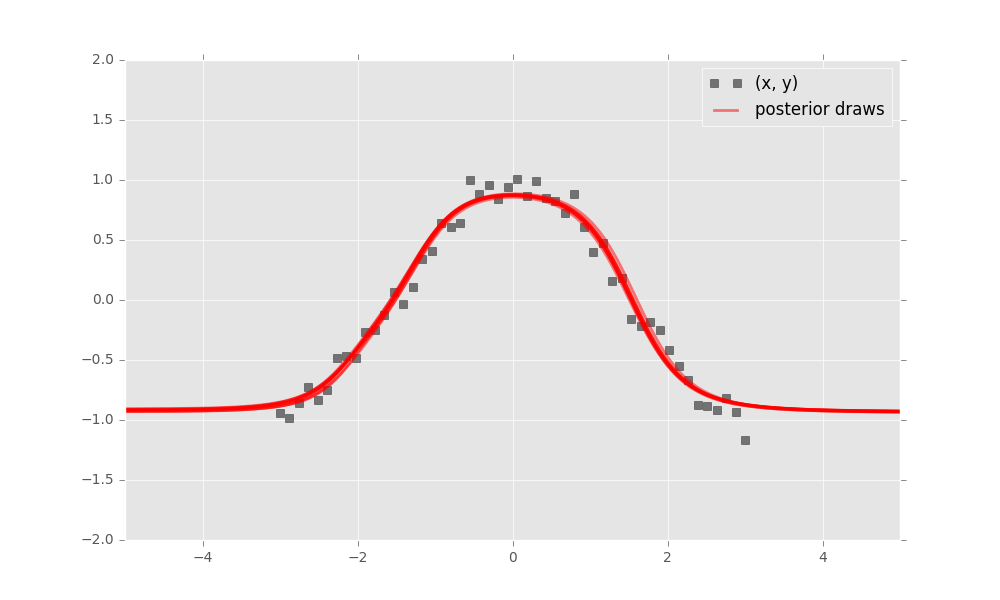
\includegraphics[width=700px]{images/getting-started-fig1.png}

The model has learned the cosine relationship between $x$ and $y$.

To learn more about Edward, \href{delving-in.html}{delve in}!

If you prefer to learn via examples, then check out some
\href{tutorials.html}{tutorials}.
